\documentclass[12pt, a4]{article}
\usepackage[utf8]{inputenc}
\usepackage{hyperref}
\hypersetup{
    colorlinks=true,
    linkcolor=black,
    filecolor=blue,      
    urlcolor=blue,
}
\usepackage{amssymb}
\usepackage[a4paper, total={6in, 9in}]{geometry}
\usepackage{graphicx}
\title{Attempting to use system identification for predicting COVID-19 cases in several countries}
\author{Cyprien Neverov\footnote{Engineering MS student at IMT Mines Ales in France, currently doing an Internship at FAU under the supervision of Prof. Zuazua. Email: cyprien.neverov@mines-ales.org}}


\begin{document}

\maketitle

In this report I describe my attempt and my current results at using data-driven system identification in order to predict the evolution of cases in several countries.

\subsection*{Introduction}

The approach described in this report relies on sparse system identification introduced in \cite{Brunton3932}. 
This is a general method for data-driven dynamic systems identification based on finding coefficients for candidate functions through optimization.


So far I only considered the simple case where we exclusively look at the total number of cases as opposed to more classic approaches where more precise quantities (susceptible, infected, recovered...) are studied like in the compartmental models. 

Let's call $y_{c,t}$ the cumulative number of cases in the country $c$ at day $t$. 
My goal is to find a function $f: \mathbb{R}^{n+1} \to \mathbb{R}$ (where $n$ is the number of indicators) such that:

$$y_{c, t+1} = f(y_{c, t}, i_{c, 1}(t), i_{c, 2}(t), i_{c, 3}(t), ... , i_{c, n}(t))$$ 

The $i_{c, k}(t), k \in \{1, 2, ..., n\}$ are the indicators for country $c$, they might be time-dependent but most of them are not. 

Here are a few examples of indicators: total population of the country, daily stringency index provided by \cite{stringency}, it informs about the severity of the anti-propagation measures, human development index, number of hospital beds per 1000 people, current health expenditure, life expectancy, percentage of the population with basic handwashing facilities including soap and water, percentage of the population that ages 80 and above and so on.
Currently, the model uses about 35 indicators that I retrieved either from the World Bank Database \cite{indicators} or from \cite{stringency}.
The indicators from the World Bank are divided into 3 categories: health, water \& sanitation and population \& age.

This approach is an attempt at combining the "dynamic systems" view with the "data scientist" philosophy. 
Usually, data scientists try to find as much data as possible and then choose the most suitable algorithms to model this data based on their knowledge, intuition or trial and error. My goal is to to do something similar but instead of using a statistical model I will try to identify the dynamics in the data.

\subsection*{Training setup}

The training dataset has 3908 training examples ($(y_t, y_{t+1})$ pairs) and 802 test examples for 105 and 26 countries\footnote{Those are the countries for which I had enough data about the virus evolution and about the indicators.} respectively. 
I used a total of 40 variables in the system. 
As candidate functions in the system identification I used polynomials of a maximum degree of 3 because for 2 the results were not satisfactory. 
In order to simplify the task all the polynomials that did not include the variable $y$ (number of cases) were excluded. 
This allowed me to get from $9880$ to $741$ candidate functions\footnote{The number of candidate functions is equal to the number of combinations with replacement: $C^R(n,r) = \frac{(n + r - 1)!}{ r! (n - 1)! }$ where $n$ is the number of variables and $r$ is the maximum degree.}.

\subsection*{Current results}

\begin{figure}[!]
  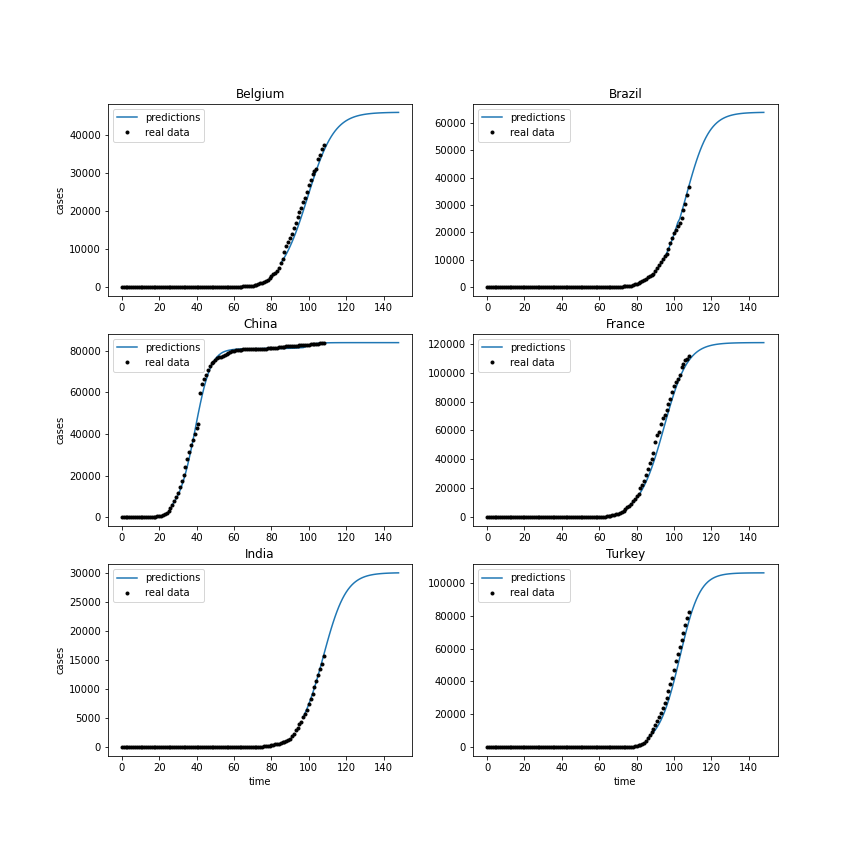
\includegraphics[width=\linewidth]{successful.png}
  \caption{Realistic-looking trajectories}
  \label{fig:successful}
\end{figure}

\begin{figure}[!]
  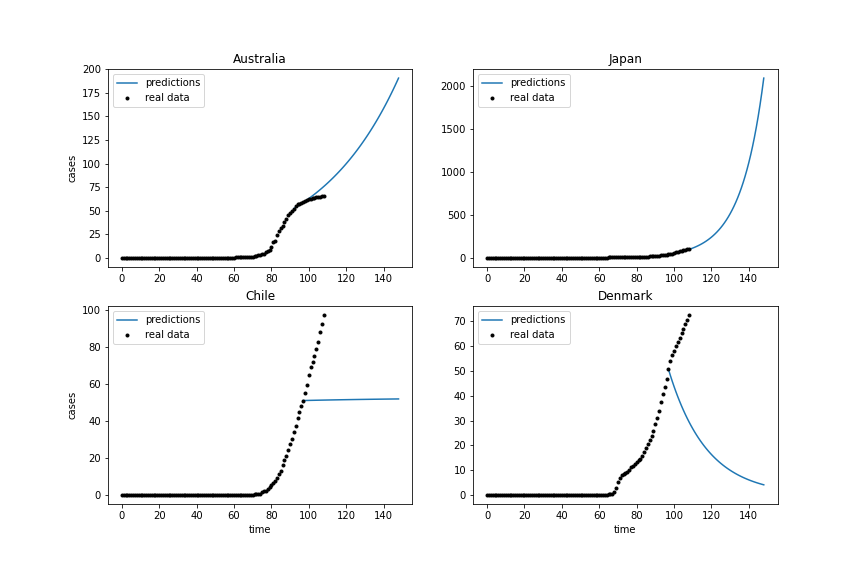
\includegraphics[width=\linewidth]{unsuccessful.png}
  \caption{Not so realistic-looking trajectories}
  \label{fig:unsuccessful}
\end{figure}

Figures \ref{fig:successful} and \ref{fig:unsuccessful} show the results of some integrations with the current setting.
All trajectories were generated with an initial value $y_0 = 5000$ cumulative cases.

In figure \ref{fig:successful} I selected some trajectories that look realistic and that seem to give predictions that make sense.
Being able to do so for all countries including those from the test set and being able to show that the predictions are close to reality would be a great outcome for this study.


Some less successful examples are displayed in figure \ref{fig:unsuccessful}. 
Australia and Japan are from the train dataset, and somehow the system did not yield any trajectories that make sense. 
Chile and Denmark are from the test dataset and they show that at the moment the model fails to generalize to examples it wasn't trained on. 
This might suggest that the 741 coefficients allow the model to overfit on the training countries. 
By overfitting I don't mean fitting to close to the real data points but learning the general evolution of a given country, and spitting it out whenever presented the same indicators rather than associating some real generalizable weight to each of the indicators.

\subsection*{Conclusion}

There is still a lot of work to do to explore the possibilities of this framework. 
What I could observe so far is that with the right settings the model is able to fit relatively well the data but no to generalize to other countries.

Also, I think that for now we have too little data for the final phases of the epidemic, only China and to a lesser extent Korea as examples.
I think that this might impact the quality of the predictions because we have a lot of data for the starting phase and very little for the final phase. 

\subsection*{Next Steps}

\begin{itemize}
  \item Add climate indicators.
  \item Try with a subset of the indicators and a higher degree of polynomials.
  \item Add other quantities (deaths, current infections, recovered...).
  \item Check if the results are similar with random indicators. 
  \item Add memory.
\end{itemize}

\bibliography{mail-refs} 
\bibliographystyle{plain}

\end{document}